\documentclass[11pt]{article}

\usepackage[strings]{underscore}
\usepackage{amsmath}
\usepackage{graphicx}
\usepackage{amssymb}

\begin{document}

\section*{Question 1}
\subsection*{Part A}

The logistic loss function for labels \{-1,1\} is the same as the logistic function 
for labels \{0,1\}. The proof is shown in~\cite{logisticloss} and summarized below.

We start with the given logistic loss equation:
\begin{equation}
		P(y | \theta, x) = \frac{1}{1+e^{-y\theta^Tx}}
		\label{eq:loss}
\end{equation}


Given that the logistic function is:
\begin{equation}
		P(y=1 | \theta, x) = \frac{1}{1+e^{-\theta^Tx}}
		\label{eq:logistic}
\end{equation}

It can be shown that given Eq(\ref{eq:logistic}), we can show that: 
\begin{equation}
		P(-x) = 1 - P(x)
\label{eq:property2}
\end{equation}

This means that:
\begin{equation}
		P(y=0 | \theta, x) = \frac{e^{-\theta^Tx}}{1+e^{-\theta^Tx}}
\end{equation}

The equations are equivalent for $y=1$. For $y=0$, it can be shown that 
$P(y=0|\theta, x)$ and $P(y=-1|\theta,x)$ are equivalent through 
Property~\ref{eq:property2}. We could also show that this leads to the same decision 
boundary. We define the boundary for logistic regression as:
\begin{align}
		\begin{split}
				\frac{\frac{1}{1+e^{-\theta^Tx}}}{\frac{e^{-\theta^Tx}}{1+e^{-\theta^Tx}}} &> 1 \rightarrow y=1 \\
		\theta^Tx &> 0 
		\end{split}
\end{align}

Likewise the boundary for logistic loss can be written as:
\begin{align}
		\begin{split}
				\frac{\frac{1}{1+e^{-\theta^Tx}}}{\frac{1}{1+e^{\theta^Tx}}} &> 1 \rightarrow y=1 \\
		\theta^Tx &> 0
		\end{split}
\end{align}

Given the logistical loss function~\ref{eq:loss}, we would try to maximize the 
probability of a vector of observed results $y$ with the likelihood function:
\begin{align}
		\begin{split}
				L(\theta) &= p(\vec{y}| \theta; X) \\
				&=\prod_{i=1}^{m}p(y^{(i)}|\theta;x^{(i)}) \\
				&=\prod_{i=1}^{m}\frac{1}{1+e^{-y\theta^Tx}}
		\end{split}
\end{align}

Taking the log likelihood and maximizing, we get the likelihood equation as:
\begin{align}
		l(\theta) = -\sum_{i=1}^{m}log(1+e^{-y\theta^Tx})
\end{align}

This is a similar form to the one provided in the question. Maximizing the log likelihood 
is also minimizing the loss function $\sum_{i=1}^{m}log(1+e^{-y\theta^Tx})$, which can be 
found in ~\cite{logisticloss}.

Getting back to the question at hand, to show that the Hessian $H$ is positive 
semidefinite, we differentiate $J(\theta)$ twice:
\begin{align}
		\begin{split}
			J(\theta) &= -\frac{1}{m}\sum_{i=1}^{m}log(1+e^{-y\theta^Tx}) \\
			          &= \frac{1}{m}\sum_{i=1}^{m}log(g(y^{(i)}\theta^Tx^{(i)}) \\ 
	         g(z) &= \frac{1}{1+e^{-z}} \\
  g(y\theta^Tx) &= \frac{1}{1+e^{-y^{(k)}\theta^Tx^{(k)}}}
		\end{split}
\end{align}
\begin{align}
		\begin{split}
		\frac{\partial J'(\theta)}{\partial \theta_j} &= -\frac{1}{m}\sum_{i=1}^{m}\frac{1}{g(y^{(k)}\theta^Tx^{(k)})}g'(y^{(k)}\theta^Tx^{(k)})y^{(k)}x^{(k)}_j \\
		&= -\frac{1}{m}\sum_{i=1}^{m}(1-g(y^{(k)}\theta^Tx^{(k)}))y^{(k)}_jx^{(k)}_j \\
		&= -\frac{1}{m}\sum_{i=1}^{m}y^{(k)}x^{(k)}_j-g(y^{(k)}\theta^Tx^{(k)})y^{(k)}x^{(k)}_j \\
		\frac{\partial J''(\theta)}{\partial \theta_j \partial \theta_i} &= -\frac{1}{m}\sum_{i=1}^{m}-y^{(k)}x^{(k)}_jg(y^{(k)}\theta^Tx^{(k)})y^{(k)}x^{(k)}_i \\
																		 &= \frac{1}{m}\sum_{i=1}^{m}y^2x_ix_j[g(y\theta^Tx)(1-g(y\theta^Tx))]
		\end{split}
\end{align}

Note in the last equation, we dropped the index k for clarity. Further since $z^THz$ can 
be re-expressed as:
\begin{align}
		\begin{split}
		z^THz &= \sum_{i}\sum_{j}(x_{ij}z_j)z_i \\
		&= \sum_{i}\sum_{j}z_i[\frac{1}{m}\sum^{m}y^2g(y\theta^Tx)(1-g(y\theta^Tx))]x_ix_jz_j
		\end{split}
\end{align}

Note that $\frac{1}{m}\sum^{m}y^2g(y\theta^Tx)(1-g(y\theta^Tx))$ is always greater than 
zero since $y^2 \geq 0$ and $0 \leq g(y\theta^Tx) \leq 1$. Therefore, we only need to 
prove that $\sum_{i}\sum_{j}z_ix_ix_jz_j>0$. We can do this by:
\begin{align}
		\begin{split}
		\sum_{i}\sum_{j}z_ix_ix_jz_j &= \sum_{i}x_iz_i\sum_{j}x_jz_j \\
		&= (x^Tz)^2 \geq 0 
		\end{split}
\end{align}

But why does proving semi-definite-ness prove convexity? We begin with the definition of 
convexity.

\textbf{Definition 1.} A function $f: \mathbb{R}^n \rightarrow \mathbb{R}$ is convex if 
its domain is a convex set and for all $x_1$, $x_2$ in its domain, and all 
$\lambda \in [0,1]$, we have:
\begin{align}
	f(\lambda x_1+(1-\lambda)x_2) \leq \lambda f(x_1) + (1-\lambda)f(x_2)
\end{align}

This equation says that an equation $f$ is convex in the range $[x_1, x_2]$ if you can 
draw a line between $f(x_1)$ and $f(x_2)$ such that the function $f$ will always be 
smaller than that. A more detailed graphical interpretation can be found 
in~\cite{convexity}.

We first prove a lemma.

\textbf{Lemma 1:} $f(x_1) \geq f(x_2) + \nabla f(x_2)^T(x_1-x_2)$, then $f$ is 
convex~\cite{characterConvexity}. 

We let $z=\lambda x_1 + (1-\lambda)x_2$. 
\begin{align}
	\begin{split}
		f(z)-f(x_2) \leq \lambda f(x_1) + (1-\lambda)f(x_2) - f(x_2) = \lambda f(x_1) - \lambda f(x_2)
	\end{split}
\end{align}

We know that the gradient $\nabla f(x_2)^T(x_1-x_2)$ can be re-expressed as
\footnote{Here $\nabla f(x_2)^T(x_1-x_2)$ is a first-order directional derivative
with expansion shown in~\cite{directionalDerivative}. It also shows why first/second-order 
expansion can be substituted by $z \in [x_1,x_2]$}

\begin{align}
	\begin{split}
		\nabla f(x_2)^T(x_1-x_2) &= \lim_{\lambda \rightarrow 0^+}\frac{f(x_2+\lambda(x_1-x_2))-f(x)}{\lambda} \\
		&= \lim_{\lambda \rightarrow 0^+}\frac{f(z)-f(x)}{\lambda} \leq f(x_2) - f(x_1)
	\end{split}
\end{align}

This implies that:
\begin{align}
	f(x_2) \geq f(z) + \nabla f(z)^T(x_2-z) \\
	f(x_1) \geq f(z) + \nabla f(z)^T(x_1-z) \\
\end{align}

Which if we multiply the first equation by $\lambda$ and second by $(1-\lambda)$ and sum 
both equations, given that we had let $z=\lambda x_1 + (1-\lambda)x_2$,  we would arrive 
at the definition of convexity in \textbf{Definition 1}.

Using \textbf{Lemma 1}, we can take the taylor expansion of $f(x_2)$:
\begin{align}
	\begin{split}
	f(x_2) = f(x_1) + \nabla f(x_1)^T(x_2-x_1) + \frac{1}{2}((x_2-x_1)^TH(z)(y-x)) \\
	\implies f(x_2) \geq f(x_1) + \nabla f(x_1)^T(x_2-x_1) \\ 
	\textnormal{if H is positive semidefinite}
	\end{split}
\end{align}
By extension of \textbf{Lemma 1}, semi-definiteness therefore proves convexity. 


\subsection*{Part B}

The co-efficients of the fit are [ 0.76037154  1.17194674 -2.6205116 ].

Several interesting caveats were discovered through mistakes. First, initially no 
parameter for y-intercept was learned. This produced pretty good results, but was 
5\% worse in accuracy than parameters that included a y-intercept (-2.6205116 above). 

Second, a programming mistake in calculating gradient 
$\frac{\partial J'(\theta)}{\partial \theta_j}$ resulted in labels that were suppose to 
be {-1} to be assigned as {1} and vice versa. Interestingly this produced the same 
boundary. The mistake was calculating $g(y^{(k)}\theta^Tx)y_j^{(k)}x_j^{(k)}$ instead of 
the correct $(1-g(y^{(k)}\theta^Tx))y_j^{(k)}x_j^{(k)}$. At first, I thought this was 
because I may have assigned the labels to probability wrong, so I simply reversed the
mappings to threshold. However, after working through the math a bit more, I realized 
I did the mapping to label correct, but somehow I was getting 12\% accuracy when I assign 
$h(\theta^Tx)>0.5 y\rightarrow1$. Upon closer inspection, the error was found.

\subsection*{Part C}
\begin{figure}
	\centering
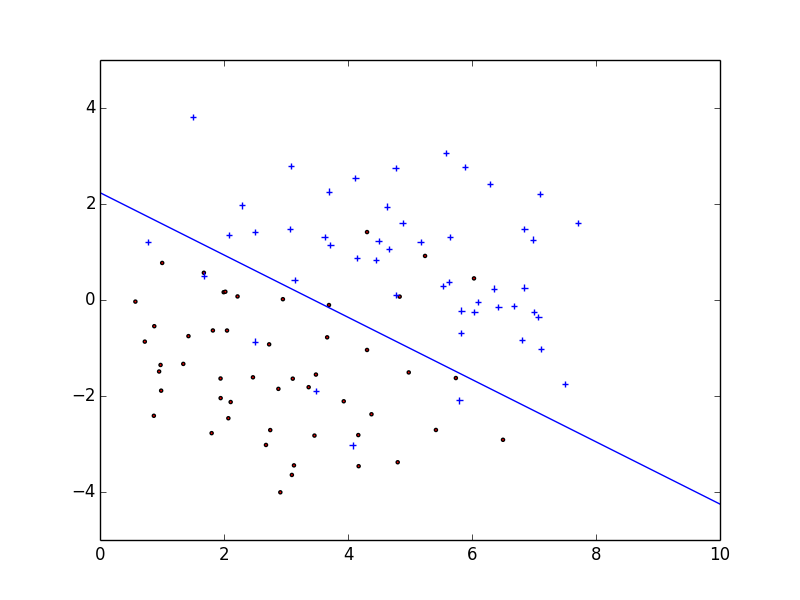
\includegraphics[width=0.75\textwidth]{../p1.png}
	\caption{ '+' indicate \{1\} labels and '.' indcate \{-1\} labels.}
	\label{fig:1c}
\end{figure}

See Figure~\ref{fig:1c}.

\section*{Question 2}
\subsection*{Part A}
\begin{align}
	\begin{split}
	p(y; \lambda) &= \frac{e^{-\lambda}\lambda^y}{y!} \\
	              &= \frac{1}{y!}e^{ylog\lambda-\lambda} \\
	 \\
	 T(y) &= y \\
	 \eta &= log\lambda \\
	 a(\eta) &= \lambda \\
	 b(y) &= \frac{1}{y!}
	\end{split}
\end{align}

\subsection*{Part B}
\begin{align}
	\begin{split}
		g(\eta) &= E[T(y);\eta] = E[y;\eta] \\
		E[y;\lambda] &= \lambda \textnormal{ and } \eta = log\lambda \implies g(\eta) = E[y;e^\eta]=e^\eta
	\end{split}
\end{align}

\subsection*{Part C}
Note: $y^{i}$ and $x^{i}$ are reduced to $y$ and $x$ for simplicity and $\eta = \theta^{T}x 
\implies \lambda = e^{\theta^Tx}$.
\begin{align}
	\begin{split}
		L(\theta) &= \sum_{i}^{m}logp(y|x;\theta) \\
							&= \sum_{i}^{m}log\frac{e^{-e^{\theta^Tx}}(e^{\theta^Tx)y}}{y!} \\
							&= \sum_{i}^{m}-e^{\theta^Tx} + y\theta^Tx - logy! \\
		\frac{\partial L(\theta)}{\partial \theta_j} &= \sum_{i}^{m}-x_je^{\theta^Tx} + yx_j \\
																								 &= \sum_{i}^{m}x_j(y-e^{\theta^Tx}) \\
	\end{split}
\end{align}

$\theta_j = \theta_j + \alpha \nabla_{\theta}l(\theta) = \theta_j + \alpha(y-e^{\theta^Tx})x_j$.

\subsection*{Part D}
\begin{align}
	\begin{split}
		l(\theta) &= logb(y) + \eta y - a(\eta) \textnormal{ with } \eta = \theta^Tx \\
		\frac{\partial l(\theta)}{\partial \theta_j} &= x_j(y - \frac{\partial a(\theta^Tx)}{\partial (\theta^Tx)}) \\
	\end{split}
\end{align}

Since $\theta_j = \theta_j + \alpha \nabla_{\theta}l(\theta) = \theta_j - \alpha(\frac{\partial 
a(\theta^Tx)}{\partial (\theta^Tx)} - y)x_j$. We only need to show that $h(x)$, the canonical 
response function (or plain english the function we use to predict), is $\frac{\partial
a(\theta^Tx)}{\partial (\theta^Tx)}$.  

\begin{align}
	\begin{split}
			        \int_{y}p(y|x;\theta)dy &= 1 \\
    \int_{y}b(y)e^{\eta^Ty-a(\eta)}dy &= 1 \\
						\int_{y}b(y)e^{\eta^Ty}dy &= e^{a(\eta)} \\
		\frac{\partial}{\partial \eta} \int_{y}b(y)e^{\eta^Ty}dy &= \frac{\partial}{\partial \eta}e^{a(\eta)} \\
		\int_{y}yb(y)e^{\eta^Ty}dy &= e^{a(\eta)}\frac{\partial a(\eta)}{\partial \eta} \\
		\int_{y}ye^{\eta^Ty-a(\eta)}dy &= \frac{\partial a(\eta)}{\partial \eta} \\
		\int_{y}yp(y|x;\theta)dy &= \frac{\partial a(\eta)}{\partial \eta} \\
		E[y|x;\theta] &= \frac{\partial a(\eta)}{\partial \eta} = h(x)
  \end{split}
\end{align}


\section*{Question 3}
\subsection*{Part A}
\begin{align}
	\begin{split}
		p(y|x; \phi, \Sigma, \mu_{-1}, \mu_{1}) &= \frac{p(x|y)p(y)}{\sum p(x|y)p(y)} \\
	\end{split}
\end{align}

\begin{align}
	\begin{split}
    p(y=1|x) &= \frac{\frac{1}{(2\pi)^{n/2}|\Sigma|^{1/2}}e^{-\frac{1}{2}(x-\mu_{1})^T\Sigma^{1}(x-\mu_{1})}\phi}
                     {\frac{1}{(2\pi)^{n/2}|\Sigma|^{1/2}}e^{-\frac{1}{2}(x-\mu_{1})^T\Sigma^{1}(x-\mu_{1})}\phi +
											\frac{1}{(2\pi)^{n/2}|\Sigma|^{1/2}}e^{-\frac{1}{2}(x-\mu_{-1})^T\Sigma^{-1}(x-\mu_{-1})}(1-\phi)} \\ 
		p(y=1|x) &= \frac{e^{-\frac{1}{2}(x-\mu_{1})^T\Sigma^{1}(x-\mu_{1})}\phi}
                     {e^{-\frac{1}{2}(x-\mu_{1})^T\Sigma^{1}(x-\mu_{1})}\phi +
											e^{-\frac{1}{2}(x-\mu_{-1})^T\Sigma^{-1}(x-\mu_{-1})}(1-\phi)} \\
		p(y=1|x) &= \frac{1}{1 + e^{ x^T\Sigma^{-1}(\mu_{-1}-\mu_{1}) - 
								\frac{1}{2}(\mu_{-1}^T\Sigma^{-1}\mu_{-1} + \mu_{1}^T\Sigma^{-1}\mu_{1}) + 
								log\frac{1-\phi}{\phi}}} \\
	\end{split}
\end{align}

\begin{align}
	\begin{split}
		p(y=-1|x) &= \frac{\frac{1}{(2\pi)^{n/2}|\Sigma|^{1/2}}e^{-\frac{1}{2}(x-\mu_{-1})^T\Sigma^{1}(x-\mu_{-1})}(1-\phi)}
                     {\frac{1}{(2\pi)^{n/2}|\Sigma|^{1/2}}e^{-\frac{1}{2}(x-\mu_{1})^T\Sigma^{1}(x-\mu_{1})}\phi +
											\frac{1}{(2\pi)^{n/2}|\Sigma|^{1/2}}e^{-\frac{1}{2}(x-\mu_{-1})^T\Sigma^{-1}(x-\mu_{-1})}(1-\phi)} \\
		p(y=-1|x) &= \frac{e^{-\frac{1}{2}(x-\mu_{-1})^T\Sigma^{-1}(x-\mu_{-1})}(1-\phi)}
                     {e^{-\frac{1}{2}(x-\mu_{1})^T\Sigma^{-1}(x-\mu_{1})}\phi +
											e^{-\frac{1}{2}(x-\mu_{-1})^T\Sigma^{-1}(x-\mu_{-1})}(1-\phi)} \\
		p(y=-1|x) &= \frac{1}{1 + e^{ x^T\Sigma^{-1}(\mu_{1}-\mu_{-1}) - 
								\frac{1}{2}(\mu_{1}^T\Sigma^{-1}\mu_{1} + \mu_{-1}^T\Sigma^{-1}\mu_{-1}) + 
								log\frac{\phi}{1-\phi}}}
	\end{split}
\end{align}

If we let $\theta=\Sigma^{-1}(\mu_1-\mu_{-1})$ and 
$\theta_0=log(\frac{\phi}{1-\phi})+\frac{1}{2}(\mu^T_{-1}\Sigma^{-1}\mu_{-1}-
\mu_1^T\Sigma^{-1}\mu_1)$, then:

\begin{align}
	\begin{split}
		p(y=1|x) &= \frac{1}{1+e^{-(\theta^Tx + \theta_0})} \\
		p(y=-1|x) &= \frac{1}{1+e^{\theta^Tx + \theta_0}}
	\end{split}
\end{align}

More succinctly, this can be written as $p(y|x)=\frac{1}{1+e^{-y(\theta^Tx + \theta_0)}}$.

\subsection*{Part B}
See Part C.
\subsection*{Part C}

\begin{align}
	\begin{split}
		\frac{\partial l(\phi, \mu_{-1}, \mu_{1}, \Sigma)}{\partial \phi} =& \sum_{i} 
				1\{y=1\}log\frac{1}{(2\pi)^{n/2}|\Sigma|^{1/2}} + \\ 
				&1\{y=-1\}log\frac{1}{(2\pi)^{n/2}|\Sigma|^{1/2}} + \\ 
				&1\{y=1\}(-\frac{1}{2}(x-\mu_1)^T\Sigma^{-1}(x-\mu_1)) + \\ 
				&1\{y=-1\}(-\frac{1}{2}(x-\mu_{-1})^T\Sigma^{-1}(x-\mu_{-1})) + \\ 
				&1\{y=1\}log\phi + 1\{y=-1\}log(1-\phi)
  \end{split}
\end{align}

For $\phi$:

\begin{align}
	\begin{split}
		\frac{\partial l(\phi, \mu_{-1}, \mu_{1}, \Sigma)}{\partial \phi} &= 
        \sum_{i}1\{y=1\}\frac{1}{\phi} - 1\{y=-1\}\frac{1}{1-\phi} \\ 
		(1-\phi)\sum_{i}1\{y=1\} &= \phi \sum_{i}1\{y=-1\} \\
        \phi &= \frac{1}{m} \sum_{i}1\{y=1\}
  \end{split}
\end{align}

For $\mu_{-1}$, $\mu_1$, and $\Sigma$, we use the following matrix gradient equations found in
the notes:

\begin{align}
	\nabla_{A}trAB &= B^T \\
  \nabla_{A^T}f(A) &= (\nabla_{A}f(A))^T \\
  \nabla_{A}trABA^TC &= CAB + C^TAB^T \\
  \nabla_{A}|A| &= |A|(A^{-1})^T
\end{align}

For $\mu_1$:
\begin{align}
	\begin{split}
		\frac{\partial l(\mu_1, \mu_{-1}, \mu_{1}, \Sigma)}{\partial \mu_1} &= 
       \sum_{i}1\{y=1\}*(-\frac{1}{2})\frac{\partial}{\partial \mu_1}tr(x-\mu_1)^T\Sigma^{-1}(x-\mu_1) \\
			 &= \sum_{i}1\{y=1\}*(-\frac{1}{2})((x-\mu_1)^T\Sigma^{-1} + (x-\mu_1)^T\Sigma^{-T})\frac{\partial}{\partial \mu_1}(x-\mu_1)^T \\
			 &= \sum_{i}1\{y=1\}(x-\mu_1)^T\Sigma^{-1} \\
		\sum_{i}1\{y=1\}x &= \sum_{i}1\{y=1\}\mu_1 \\
		\mu_1 &= \frac{\sum_{i}1\{y=1\}x}{\sum_{i}1\{y=1\}}
	\end{split}
\end{align}

For $\mu_{-1}$:
\begin{align}
	\begin{split}
		\frac{\partial l(\mu_1, \mu_{-1}, \mu_{1}, \Sigma)}{\partial \mu_{-1}} &= 
			 \sum_{i}1\{y=-1\}*(-\frac{1}{2})\frac{\partial}{\partial \mu_{-1}}tr(x-\mu_{-1})^T\Sigma^{-1}(x-\mu_{-1}) \\
			 &= \sum_{i}1\{y=-1\}*(-\frac{1}{2})((x-\mu_{-1})^T\Sigma^{-1} + (x-\mu_{-1})^T\Sigma^{-T})\frac{\partial}{\partial \mu_{-1}}(x-\mu_{-1})^T \\
			 &= \sum_{i}1\{y=-1\}(x-\mu_{-1})^T\Sigma^{-1} \\
		\sum_{i}1\{y=-1\}x &= \sum_{i}1\{y=-1\}\mu_{-1} \\
		\mu_{-1} &= \frac{\sum_{i}1\{y=-1\}x}{\sum_{i}1\{y=-1\}}
	\end{split}
\end{align}

For $\Sigma$:
\begin{align}
	\begin{split}
		\frac{\partial l(\mu_1, \mu_{-1}, \mu_{1}, \Sigma)}{\partial \Sigma^{-1}} =& -\frac{1}{2}\sum_{i} 
		1\{y=1\}\Sigma + 1\{y=-1\}\Sigma + \\
		&1\{y=1\}(x-\mu_1)(x-\mu_1)^T + 1\{y=-1\}(x-\mu_{-1})(x-\mu_{-1})^T \\
		m\Sigma =& \sum_{i}(x-\mu_1)(x-\mu_1)^T + (x-\mu_{-1})(x-\mu_{-1})^T \\
		\Sigma =& \frac{1}{m}\sum_{i}(x-\mu_y)(x-\mu_y)^T 
	\end{split}
\end{align}

For $\Sigma$ above, we needed to use several interesting properties:
\begin{enumerate}
	\item determinant of matrix inverse is inverse of the matrix determinant $|\Sigma|= \frac{1}{\Sigma^{-1}}$
	\item trace of matrix cyclically permutate $tr(ABC)=tr(BCA)=tr(CAB)$
	\item matrix $\Sigma$ is symmetric
\end{enumerate}

\section*{Question 4}
\subsection*{Part A}
Newton's method is defined as $x^{i+1}=x^{i}-\frac{f'(x)}{f''(x)}$.
For $g(z)$:
\begin{align}
	\begin{split}
		z^{i+1} &= z^{i}-\frac{g'(z)}{g''(z)} \\
		g'(z) &= f'(Az)\frac{\partial (Az)}{\partial z}=Af'(Az) \\
	  g''(z) &= f''(Az) = A^2f''(Az) = A^2g(z) \\
		z^{i+1} &= z^{i} - \frac{Af'(Az)}{A^2f''(Az)} \\
	\end{split}
\end{align}

We assume $z^{i}=A^{-1}x^{i}$ and know that the base case $z^{0}$ is true. We only need to prove
that $z^{i+1}=A^{-1}x^{i+1}$. Since $\frac{f'(x)}{f''(x)}=x^{i}-x^{i+1}$:
\begin{align}
	\begin{split}
		z^{i+1} &= z^{i} - (x^{i}-x^{i+1})A^{-1} \\
		        &= A^{-1}x^{i+1}
	\end{split}
\end{align}

Therefore Newton's method is invariant to linear re-parameterization. 

\subsection*{Part B}
Gradient descent is defined as $x^{i+1}=x^{i}-\alpha f'(x^{i})$. Since $x^{i}=Az^{i}$ and 
$f'(x^{i})=\frac{x^{i}-x^{i+1}}{\alpha}$:
\begin{align}
	\begin{split}
		z^{i+1} &= z^{i}-\alpha Af'(Az^{i}) \\
		z^{i+1} &= A^{-1}x^{i} - Ax^{i} + Ax^{i+1}
	\end{split}
\end{align}

Gradient descent is not invariant to linear re-parameterization.

\section*{Question 5}
\subsection*{Part A}
\subsubsection*{$i)$ }
\begin{align}
	\begin{split}
		J(\theta) &= (X\theta-y)^TW(X\theta-y) \\
							&= (\begin{bmatrix} X^{0} \\ X^{1} \\ \vdots \\ X^{i} \end{bmatrix}
								\begin{bmatrix} \theta_0 \\ \theta_1 \\ \vdots \\ \theta_n \end{bmatrix} -
									\begin{bmatrix} y^{0} \\ y^{1} \\ \vdots \\ y{i} \end{bmatrix})^T
								 (\begin{bmatrix} \frac{1}{2}w^{0} \\ & \frac{1}{2}w^{1} \\ & & \ddots \\ & & & \frac{1}{2}w^{i} \end{bmatrix})
								 (\begin{bmatrix} X^{0} \\ X^{1} \\ \vdots \\ X^{i} \end{bmatrix}
								  \begin{bmatrix} \theta_0 \\ \theta_1 \\ \vdots \\ \theta_n \end{bmatrix} -
									\begin{bmatrix} y^{0} \\ y^{1} \\ \vdots \\ y{i} \end{bmatrix}) \\
							&= \frac{1}{2} \begin{bmatrix} \theta^{T}x^{0} & \theta^{T}x^{1} & \cdots & \theta^{T}x^{i} \end{bmatrix} 
								 \begin{bmatrix} w^{0}(\theta^Tx^{0}-y^{0}) \\ w^{1}(\theta^Tx^{1}-y^{1}) \\ \vdots \\ w^{i}(\theta^Tx^{i}-y^{i}) \end{bmatrix} \\
							&= \frac{1}{2} \sum_i (\theta^Tx^{i}-y^{i})w^{i}(\theta^Tx^{i}-y^{i}) \\
							&= \frac{1}{2} \sum_i w^{i}(\theta^Tx^{i}-y^{i})^2
		\end{split}
\end{align}
\subsubsection*{$ii)$ }
\begin{align}
	\begin{split}
		\nabla_\theta J(\theta) &= \frac{1}{2} \nabla_\theta (X\theta-y)^TW(X\theta-y) \\
													  &= \frac{1}{2} \nabla_\theta \theta^TX^TWX\theta - \theta^TX^TWy - y^TWX\theta + y^TWy \\
														&= \frac{1}{2} ( (\theta^TX^TWX)^T + \theta^TX^TW^TX- (X^TWy) - y^TWX ) \\
		\end{split}
\end{align}

We set $\nabla_\theta J(\theta)=0$, and since $W$ is a diagonal matrix $W^T = W$:

\begin{align}
	\begin{split}
		2X^TWX\theta &= 2X^TWy \\
					\theta &= (X^TWX)^{-1}X^TW^Ty 
		\end{split}
\end{align}

\subsubsection*{$iii)$ }

\begin{align}
	\begin{split}
		l(\theta) &= log \prod_i \frac{1}{\sqrt{2\pi}\sigma^{i}}e^{-\frac{(y^{i}-\theta^Tx^{i})^2}{2(\sigma^{i})^2}} \\
							&= - \sum_i log \sqrt{2\pi}\sigma^{i} - \frac{(y^{i}-\theta^Tx^{i})^2}{2(\sigma^{i})^2} \\
		\frac{\partial l'(\theta)}{\partial \theta} &= \frac{\partial l'(\theta)}{\partial \theta} \frac{1}{2} \sum_i \frac{1}{\sigma^{(i)2}}(\theta^Tx^{i} - y^{i})^2  	
	\end{split}
\end{align}

In this case, the problem of normal distributed samples with differing variances reduce to a 
weighted linear regression problem where $w^{i}=\frac{1}{(\sigma^{i})^2}$.


\subsection*{Part B}
\subsubsection*{$i)$}
\begin{figure}
	\centering
	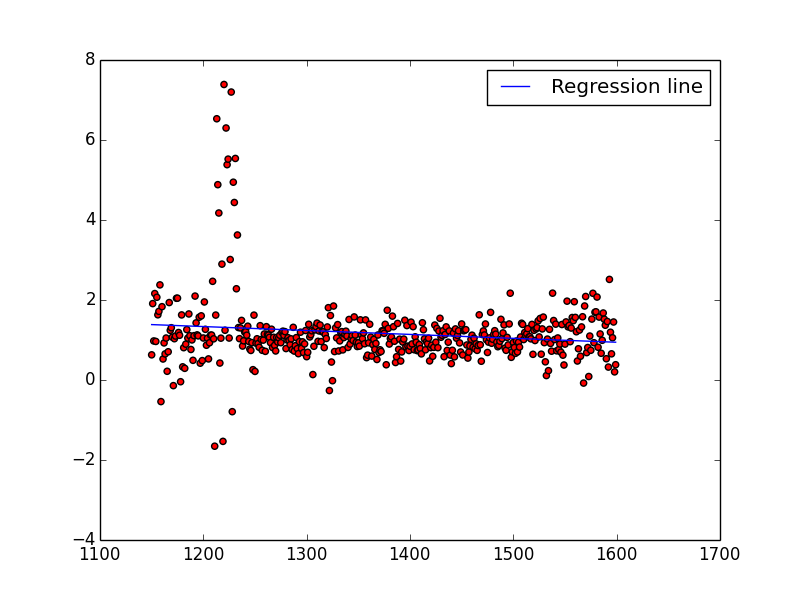
\includegraphics[width=0.75\textwidth]{../p5b1.png}
	\caption{ Linear Regression of first training sample of quasar data. $y=\theta^Tx$ where $\theta=(X^TX)^{-1}X^Ty$}
	\label{fig:5b1}
\end{figure}

See Figure~\ref{fig:5b1}.

\subsubsection*{$ii)$}
\begin{figure}
	\centering
	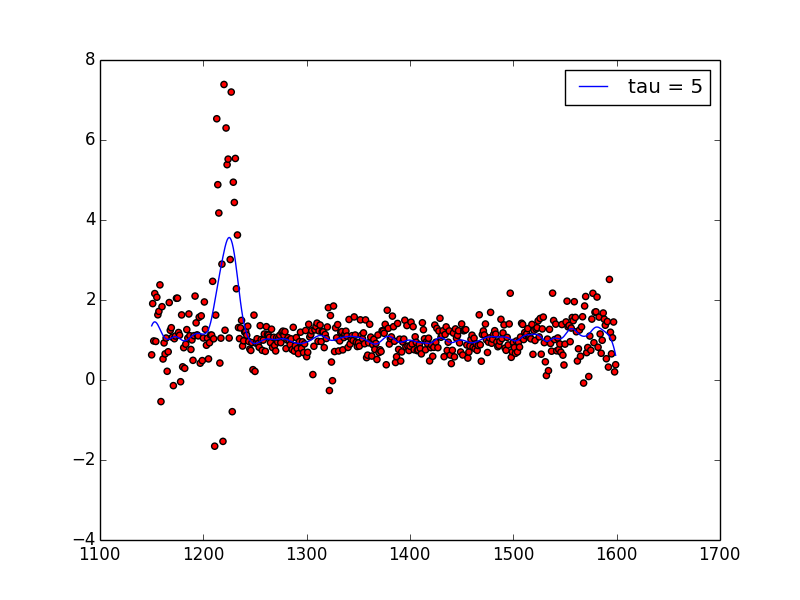
\includegraphics[width=0.75\textwidth]{../p5b2.png}
	\caption{ Weighted Linear Regression of first training sample of quasar data. $y=\theta^T(x)x$ where $\theta=(X^TWX)^{-1}X^TW^Ty$}
	\label{fig:5b2}
\end{figure}

See Figure~\ref{fig:5b2}.

\subsubsection*{$iii)$}
\begin{figure}
	\centering
	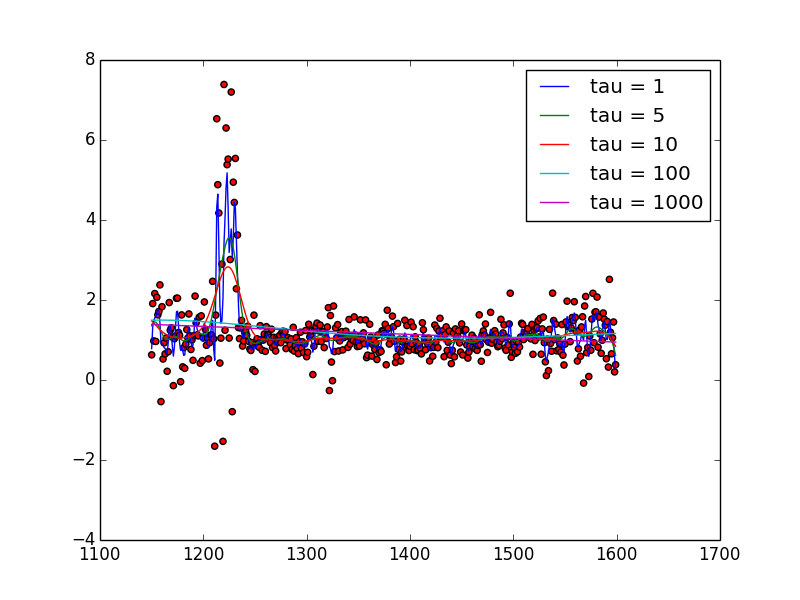
\includegraphics[width=0.75\textwidth]{../p5b3.png}
	\caption{ Weighted Linear Regression of first training sample of quasar data. $y=\theta^T(x)x$ where $\theta=(X^TWX)^{-1}X^TW^Ty$. $\tau = 1,10,100,1000$ . }
	\label{fig:5b3}
\end{figure}

See Figure~\ref{fig:5b3}. The higher the value $\tau$, the closer the estimated curve $y=h(x)$ tracks
the data points. 

\subsection*{Part C}
\subsubsection*{$i)$}

See Q5.py.

\subsubsection*{$ii)$}

See Q5.py. Training set error 1.0664.

\subsubsection*{$iii)$}

See Q5.py and Figure~\ref{fig:5c3-1} and~\ref{fig:5c3-6}. Test set error 2.7100.

\begin{figure}
	\centering
	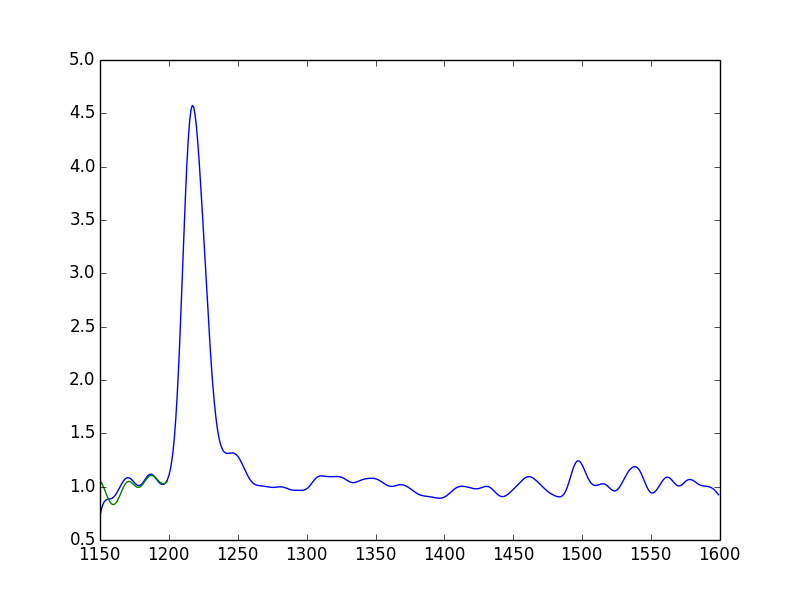
\includegraphics[width=0.75\textwidth]{../p5c3-1.png}
	\caption{ Weighted Linear Regression of test sample 1 of quasar data. }
	\label{fig:5c3-1}
\end{figure}

\begin{figure}
	\centering
	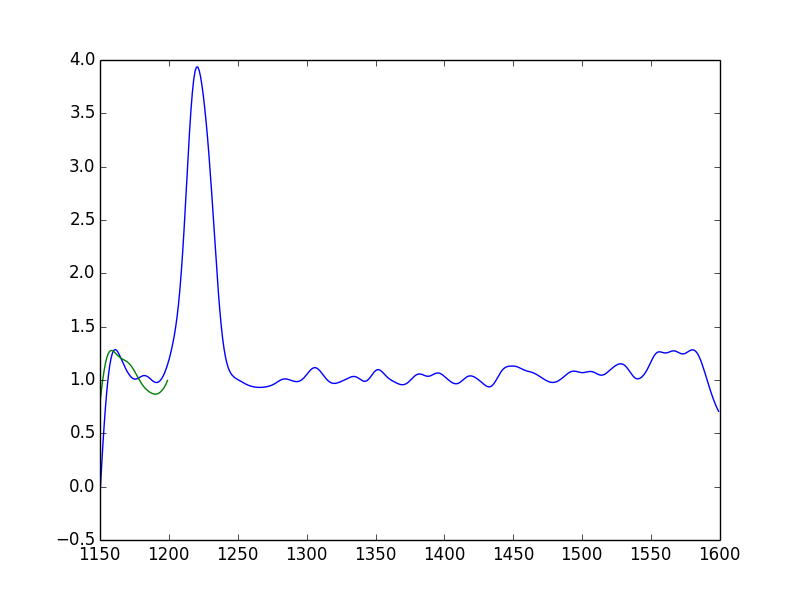
\includegraphics[width=0.75\textwidth]{../p5c3-6.png}
	\caption{ Weighted Linear Regression of test sample 1 of quasar data. }
	\label{fig:5c3-6}
\end{figure}

\bibliographystyle{abbrv}
\bibliography{solutions}

\end{document}
